\chapter{Interfases, tensioactivos y coloides}\label{ch:b3:colloids}

La mayonesa es aceite disperso en gotitas de unos pocos micrómetros en un poco de
agua y vinagre, mantenidas separadas por la lecitina y las proteínas de la yema de huevo. Si se bate
demasiado deprisa al principio, o si se vierte el aceite demasiado rápido, se corta en una
capa aceitosa y otra acuosa: las gotitas se fusionan, y la energía que las mantenía
separadas desaparece. La leche, la niebla, la tinta, la pintura, la sangre y el agua turbia de un río son
el mismo tipo de materia, partículas o gotitas mucho mayores que las moléculas y
mucho menores que cualquier cosa que vea el ojo, tan numerosas que la mayor parte de sus moléculas
están cerca de una interfase. Este capítulo trata la energía de las interfases, las
moléculas que la rebajan, los \omterm{def:b3:colloids:colloid}{coloides} que las interfases hacen posibles y lo que
mantiene dispersos los \omterm{def:b3:colloids:colloid}{coloides} o los hace coagular.

\begin{recall}
El volumen del primer año llamó anfífila a una molécula con una cabeza hidrófila y una
cola hidrófoba, y describió las interacciones de London y la permitividad relativa
de los disolventes; la parte del año 11 del primer volumen presentó las \omterm{def:b3:colloids:micelle}{micelas}
del jabón. El volumen del segundo año definió el potencial químico, la fuerza iónica y la
actividad. El \cref{ch:b3:surfaces-catalysis} trató la \omterm{def:b3:surfaces-catalysis:adsorption}{adsorción} sobre sólidos, y
el \cref{ch:b3:electrode-kinetics}, la \omterm{def:b3:electrode-kinetics:double-layer}{doble capa eléctrica} y su \omterm{def:b3:electrode-kinetics:double-layer}{longitud de
Debye}. De la física: el movimiento browniano y la presión en el interior de una superficie
curva.
\end{recall}

\begin{omfigure}
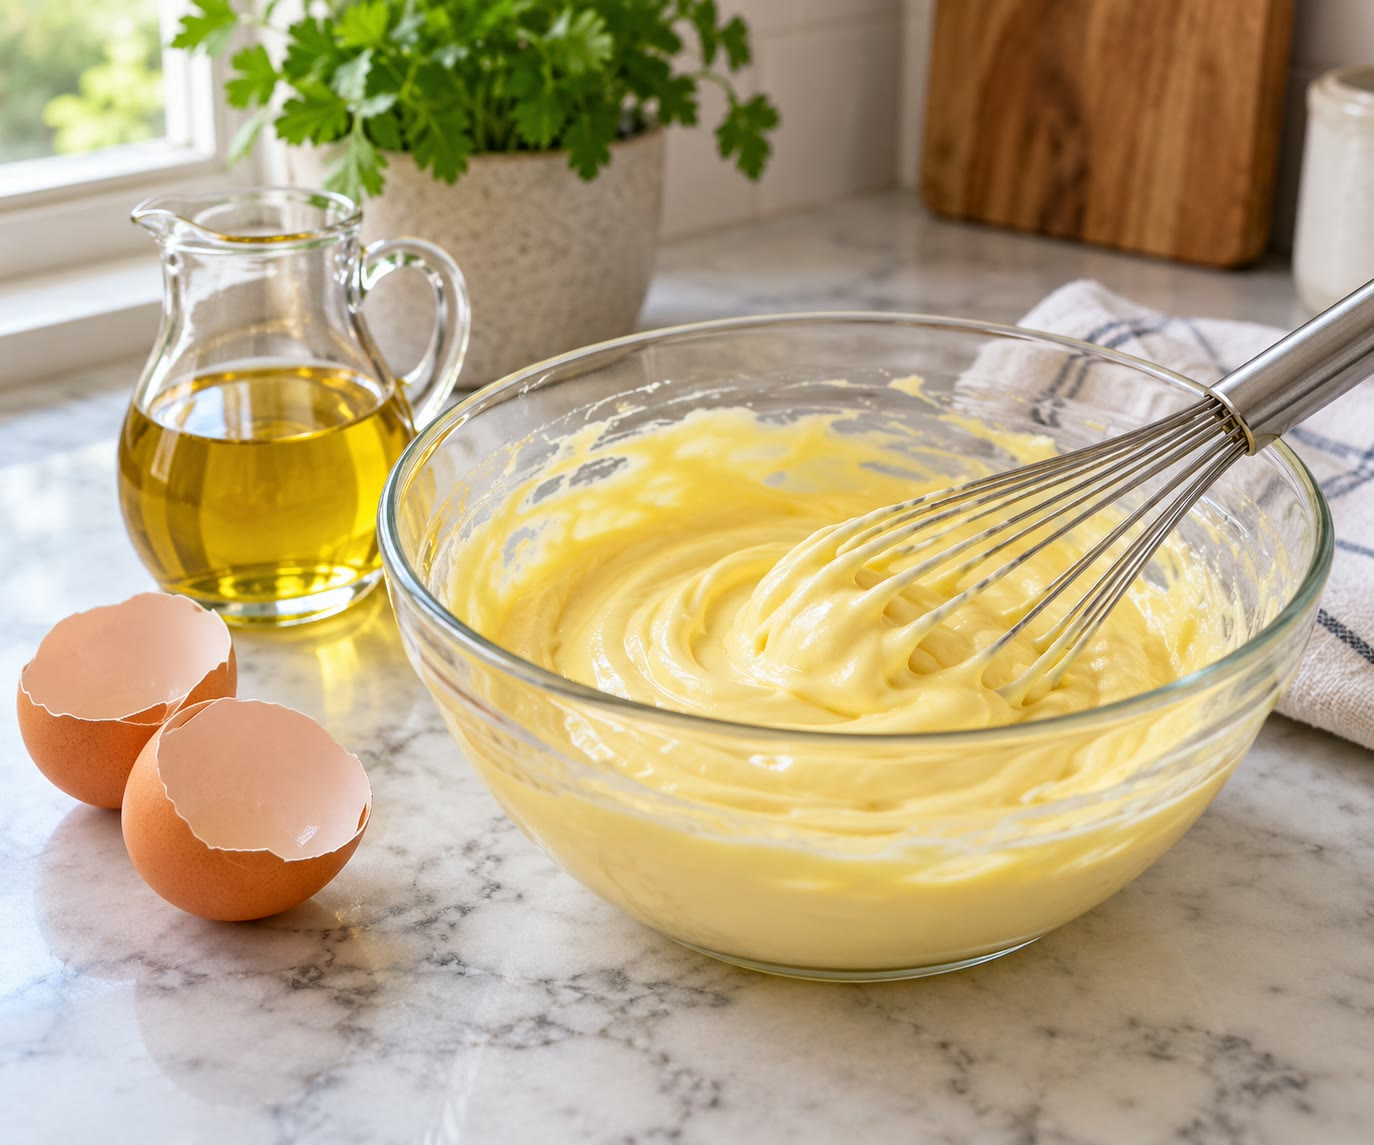
\includegraphics[width=0.6\linewidth]{images/book4/ai/b3-17-mayonnaise.jpg}

{\small Mayonesa batida: una \omterm{def:b3:colloids:colloid}{emulsión} de gotitas de aceite en agua,
estabilizada por los \omterm{def:b3:colloids:surfactant}{tensioactivos} de la yema de huevo.}
\end{omfigure}

\section{Interfases y tensión superficial}

Una molécula en el seno de un líquido es atraída por igual en todas las direcciones; en
la superficie pierde parte de sus vecinas. Crear superficie cuesta energía.

\begin{definition}[Tensión superficial]\label{def:b3:colloids:surface-tension}
La \emph{tensión superficial}\index{tension superficial@tensión superficial} $\gamma$ de un líquido es la energía de
Gibbs necesaria para crear una unidad de área de su superficie a temperatura, presión y
composición constantes: $\gamma = (\partial G/\partial A)_{T,p,n}$, en \unit{J.m^{-2}} $=$ \unit{N.m^{-1}}. Para una
interfase entre dos fases es la tensión interfacial.
\end{definition}

El agua, cohesionada por enlaces de hidrógeno, tiene una \omterm{def:b3:colloids:surface-tension}{tensión superficial} alta: \qty{72.0}{mN/m}
a \qty{25}{\celsius}. Los alcanos tienen unos 20, y el mercurio, unos 480.

\begin{proposition}[Presión de Laplace]\label{prop:b3:colloids:laplace}
La presión en el interior de una gota o una burbuja esférica de radio $r$ supera la
presión exterior en
\[
  \Delta p = \frac{2\gamma}{r} .
\]
\end{proposition}

\begin{proof}
Se aumenta el radio en $\dd r$ en el equilibrio: el trabajo de la diferencia de
presión, $\Delta p\,4\pi r^2\dd r$, es igual al aumento de la energía de Gibbs superficial, $\gamma\,8\pi r\,\dd r$.
\end{proof}

\begin{definition}[Ángulo de contacto, mojado]\label{def:b3:colloids:wetting}
El \emph{ángulo de contacto}\index{angulo de contacto@ángulo de contacto} $\theta$ de una gota sobre un sólido es el ángulo,
medido a través del líquido, entre la superficie del sólido y la superficie del líquido
en la línea donde se encuentran el sólido, el líquido y el vapor. Un líquido \emph{moja}\index{mojado}
el sólido cuando $\theta < 90^\circ$, y se extiende por completo cuando $\theta = 0$.
\end{definition}

\begin{theorem}[Ecuación de Young]\label{thm:b3:colloids:young}
En el equilibrio, las tres tensiones interfaciales y el \omterm{def:b3:colloids:wetting}{ángulo de contacto} cumplen
\[
  \gamma_{\mathrm{SV}} = \gamma_{\mathrm{SL}} + \gamma_{\mathrm{LV}}\cos\theta .
\]
Es la \emph{ecuación de Young}\index{ecuacion de Young@ecuación de Young}.
\end{theorem}

\begin{proof}
Se desplaza la línea de contacto hacia fuera en $\dd x$ (por unidad de longitud de línea): una
interfase sólido--vapor de área $\dd x$ se sustituye por una interfase sólido--líquido, y la
interfase líquido--vapor crece en $\dd x\cos\theta$. La energía de Gibbs varía en
$(\gamma_{\mathrm{SL}} - \gamma_{\mathrm{SV}} + \gamma_{\mathrm{LV}}\cos\theta)\dd x$, que es nula en el equilibrio.
\end{proof}

\begin{omfigure}
\begin{tikzpicture}[font=\small, >=Stealth]
  \fill[black!12] (-3.6,-0.5) rectangle (3.6,0);
  \draw[thick] (-3.6,0) -- (3.6,0);
  \node[anchor=north] at (2.6,-0.05) {sólido};
  \fill[omWater!60] (-2.0,0) arc[start angle=160, end angle=20, radius=2.13] -- cycle;
  \draw[thick, omDef] (-2.0,0) arc[start angle=160, end angle=20, radius=2.13];
  % circle centre 0.73 below the solid: a cap smaller than a hemisphere, contact angle 90 - 20 = 70 deg;
  % at the right contact point the liquid surface leaves at 110 deg (up and to the left)
  \draw[->, thick, omThm] (2.0,0) -- ++(110:1.3) node[anchor=south] {$\gamma_{\mathrm{LV}}$};
  \draw[->, thick] (2.0,0) -- (3.3,0) node[anchor=south] {$\gamma_{\mathrm{SV}}$};
  \draw[->, thick] (2.0,0) -- (0.7,0) node[anchor=north, yshift=-1pt] {$\gamma_{\mathrm{SL}}$};
  \draw (1.45,0) arc[start angle=180, end angle=110, radius=0.55];
  \node at (1.33,0.42) {$\theta$};
  \node at (0,0.6) {líquido};
  \node at (-2.8,1.4) {vapor};
\end{tikzpicture}

{\small Una gota sésil y las tres tensiones que tiran de su línea de contacto: el
balance de sus componentes a lo largo del sólido da la \omterm{thm:b3:colloids:young}{ecuación de Young}; aquí $\theta
\approx 70^\circ$, un líquido que \omterm{def:b3:colloids:wetting}{moja} parcialmente.}
\end{omfigure}

\begin{theorem}[Ecuación de Kelvin]\label{thm:b3:colloids:kelvin}
La presión de vapor de una gota esférica de radio $r$ supera a la del líquido
plano, $p^*$:
\[
  \ln\frac{p}{p^*} = \frac{2\gamma V_{\mathrm m}}{rRT},
\]
con $V_{\mathrm m}$ el volumen molar del líquido. Es la \emph{ecuación de
Kelvin}\index{ecuacion de Kelvin@ecuación de Kelvin}.
\end{theorem}

\begin{proof}
El líquido de la gota está sometido a la presión adicional $2\gamma/r$, que eleva su
potencial químico en $V_{\mathrm m}\,2\gamma/r$ (con $(\partial\mu/\partial p)_T = V_{\mathrm m}$ y el líquido incompresible).
El vapor en equilibrio con él debe tener su potencial químico elevado en
la misma cantidad: $RT\ln(p/p^*) = 2\gamma V_{\mathrm m}/r$.
\end{proof}

Para una gotita de agua de \qty{10}{nm} de radio a \qty{25}{\celsius}, $2\gamma V_{\mathrm m}/rRT = 0.105$: su presión
de vapor es un 11\,\% mayor que la del agua plana. Las gotitas pequeñas se evaporan mientras
las grandes crecen, y las nubes necesitan núcleos para formarse; lo mismo vale para la
solubilidad de los cristales pequeños.

\begin{definition}[Maduración de Ostwald]\label{def:b3:colloids:ripening}
La \emph{maduración de Ostwald}\index{maduracion de Ostwald@maduración de Ostwald} es el crecimiento de las partículas
o gotitas más grandes de una dispersión a expensas de las más pequeñas,
impulsado por la mayor solubilidad o presión de vapor de las partículas pequeñas.
\end{definition}

\section{Tensioactivos y micelas}

\begin{definition}[Tensioactivo]\label{def:b3:colloids:surfactant}
Un \emph{tensioactivo}\index{tensioactivo} (agente de superficie) es una molécula
anfífila que se adsorbe en las interfases y rebaja su tensión. Es un
\emph{tensioactivo aniónico}\index{tensioactivo anionico@tensioactivo aniónico} si su cabeza es un anión (dodecilsulfato
de sodio, jabones), un \emph{tensioactivo catiónico}\index{tensioactivo cationico@tensioactivo catiónico}
si es un catión (sales de amonio cuaternario), y un \emph{tensioactivo no
iónico}\index{tensioactivo no ionico@tensioactivo no iónico} si la cabeza es un grupo polar neutro (una
cadena de unidades de óxido de etileno).
\end{definition}

\begin{definition}[Concentración de exceso superficial]\label{def:b3:colloids:surface-excess}
La \emph{concentración de exceso superficial}\index{concentracion de exceso superficial@concentración de exceso superficial} $\Gamma$ de un
soluto es la cantidad de soluto en la interfase por unidad de área, por encima de
la que contendría el mismo volumen si la concentración del seno de la disolución se mantuviera hasta
la interfase.
\end{definition}

\begin{theorem}[Isoterma de adsorción de Gibbs]\label{thm:b3:colloids:gibbs-adsorption}
Para una disolución diluida de un soluto no iónico de concentración $c$,
\[
  \Gamma = -\frac{1}{RT}\frac{\dd\gamma}{\dd\ln c};
\]
para un \omterm{def:b3:colloids:surfactant}{tensioactivo} iónico 1:1 sin sal añadida, $RT$ se sustituye por $2RT$. Es
la \emph{isoterma de adsorción de Gibbs}\index{isoterma de adsorcion de Gibbs@isoterma de adsorción de Gibbs}.
\end{theorem}

\begin{proof}
Para la interfase, el análogo de la relación de Gibbs--Duhem a $T$ y
$p$ constantes es $\dd\gamma = -\sum_i\Gamma_i\,\dd\mu_i$ (la energía de Gibbs superficial $\gamma A$ desempeña el papel de $G$;
se admite). Eligiendo la superficie divisoria de modo que el disolvente no tenga exceso,
$\dd\gamma = -\Gamma\,\dd\mu$, y en una disolución diluida $\dd\mu = RT\,\dd\ln c$. Para un \omterm{def:b3:colloids:surfactant}{tensioactivo} iónico,
el catión y el anión se adsorben ambos con el mismo exceso y $\dd\mu$ pasa a ser
$2RT\,\dd\ln c$.
\end{proof}

Un \omterm{def:b3:colloids:surfactant}{tensioactivo} cuya \omterm{def:b3:colloids:surface-tension}{tensión superficial} disminuye linealmente con $\ln c$ tiene un exceso
superficial constante: la interfase está saturada, y $1/(\Gamma N_A)$ es el área ocupada por
una molécula adsorbida.

\begin{method}[Área por molécula a partir de una pendiente $\gamma$--$\ln c$]\label{met:b3:colloids:surface-excess}
\begin{enumerate}
  \item Medir $\gamma$ en función de $c$ por debajo de la CMC; representar $\gamma$ en función de $\ln c$.
  \item Tomar la pendiente de la parte lineal justo por debajo de la CMC; $\Gamma = -\text{pendiente}/(nRT)$, con $n
        = 1$ para un \omterm{def:b3:colloids:surfactant}{tensioactivo no iónico} y 2 para uno iónico 1:1 sin sal.
  \item Área por molécula $= 1/(\Gamma N_A)$; los valores típicos van de 0.3 a \qty{0.6}{nm^2}.
\end{enumerate}
\end{method}

\begin{definition}[Micela, concentración micelar crítica, número de agregación]\label{def:b3:colloids:micelle}
Una \emph{micela}\index{micela} es un agregado de moléculas de \omterm{def:b3:colloids:surfactant}{tensioactivo} en disolución
cuyas colas hidrófobas forman un núcleo de tipo líquido protegido del agua por las
cabezas. La \emph{concentración micelar crítica}\index{concentracion micelar critica@concentración micelar crítica}
(CMC) es la concentración por encima de la cual se forman micelas; su
número medio de moléculas es el \emph{número de agregación}\index{numero de agregacion@número de agregación}.
\end{definition}

\begin{proposition}[Cambios de pendiente en la CMC]\label{prop:b3:colloids:cmc-break}
Por encima de la CMC, la concentración de \omterm{def:b3:colloids:surfactant}{tensioactivo} libre, y con ella la \omterm{def:b3:colloids:surface-tension}{tensión
superficial} y la presión osmótica, se mantienen casi constantes; las propiedades que dependen
de las moléculas libres cambian de pendiente en la CMC.
\end{proposition}

\begin{proof}[Demostración parcial]
Se tratan las \omterm{def:b3:colloids:micelle}{micelas} como una fase aparte: el \omterm{def:b3:colloids:surfactant}{tensioactivo} añadido pasa a las \omterm{def:b3:colloids:micelle}{micelas} en cuanto
el potencial químico de las moléculas libres alcanza el de una molécula en una
\omterm{def:b3:colloids:micelle}{micela}, y este potencial químico, y por tanto la concentración libre, queda entonces
fijo. La \omterm{def:b3:colloids:surface-tension}{tensión superficial}, fijada por las moléculas libres a través de la isoterma de
Gibbs, deja de disminuir; la conductividad sigue aumentando, pero más despacio, ya que
las \omterm{def:b3:colloids:micelle}{micelas} llevan menos carga por \omterm{def:b3:colloids:surfactant}{tensioactivo} que los iones libres (parte de sus
contraiones están ligados). El modelo es un límite, ya que las \omterm{def:b3:colloids:micelle}{micelas} de tamaño finito
se forman en un intervalo estrecho de concentración (se admite).
\end{proof}

\begin{method}[La CMC a partir de un cambio de pendiente]\label{met:b3:colloids:cmc}
\begin{enumerate}
  \item Medir la \omterm{def:b3:colloids:surface-tension}{tensión superficial} (o, para un \omterm{def:b3:colloids:surfactant}{tensioactivo} iónico, la
        conductividad) en un intervalo de concentraciones que abarque la CMC
        esperada.
  \item Ajustar rectas a las dos ramas ($\gamma$ en función de $\log c$, o $\kappa$ en función de $c$).
  \item Su intersección es la CMC.
\end{enumerate}
\end{method}

\begin{omfigure}
\begin{tikzpicture}
\begin{axis}[name=gm, width=0.47\linewidth, height=5.2cm, xmin=-5, xmax=-1.5, ymin=30, ymax=76,
  axis lines=left, xlabel={$\log(c/\unit{mol.L^{-1}})$}, ylabel={$\gamma$ / \unit{mN.m^{-1}}},
  tick label style={font=\small}, label style={font=\small}]
\addplot[omDef, very thick] table[x=logc, y=gamma_mN] {figdata/out/bachelor-3-surfactant-cmc-gamma.dat};
\draw[black!40, dashed] (axis cs:-2.086,30) -- (axis cs:-2.086,70);
\node[font=\scriptsize, anchor=south west] at (axis cs:-2.05,45) {CMC};
\end{axis}
\begin{axis}[at={(gm.east)}, anchor=west, xshift=1.4cm, width=0.47\linewidth, height=5.2cm,
  xmin=0, xmax=20, ymin=0, ymax=1.0, axis lines=left, xlabel={$c$ / mM},
  ylabel={$\kappa$ / \unit{mS.cm^{-1}}}, tick label style={font=\small}, label style={font=\small}]
\addplot[omThm, very thick] table[x=c_mM, y=kappa] {figdata/out/bachelor-3-surfactant-cmc-kappa.dat};
\draw[black!40, dashed] (axis cs:8.2,0) -- (axis cs:8.2,0.9);
\node[font=\scriptsize, anchor=south west] at (axis cs:8.4,0.15) {CMC};
\end{axis}
\end{tikzpicture}

{\small Un \omterm{def:b3:colloids:surfactant}{tensioactivo} iónico modelo con la CMC del dodecilsulfato de sodio,
\qty{8.2}{mM} a \qty{25}{\celsius}. Izquierda: la \omterm{def:b3:colloids:surface-tension}{tensión superficial} disminuye con $\log c$, linealmente justo por debajo de
la CMC (una interfase saturada, con unos \qty{0.6}{nm^2} por molécula), y después se mantiene
constante. Derecha: la conductividad sube con menos pendiente por encima de la CMC.}
\end{omfigure}

\begin{definition}[Parámetro de empaquetamiento]\label{def:b3:colloids:packing}
El \emph{parámetro de empaquetamiento}\index{parametro de empaquetamiento@parámetro de empaquetamiento} de un \omterm{def:b3:colloids:surfactant}{tensioactivo} es $P =
v/(a_0l)$, donde $v$ es el volumen de su cola hidrófoba, $l$ la longitud de la
cola extendida y $a_0$ el área óptima por grupo de cabeza en la superficie del
agregado.
\end{definition}

\begin{proposition}[Forma de los agregados]\label{prop:b3:colloids:packing}
Las \omterm{def:b3:colloids:micelle}{micelas} esféricas necesitan $P \le \frac13$, las \omterm{def:b3:colloids:micelle}{micelas} cilíndricas $\frac13 < P \le \frac12$, y las bicapas planas
(vesículas, membranas) $\frac12 < P \le 1$; $P > 1$ da estructuras invertidas.
\end{proposition}

\begin{proof}
En una esfera de radio $R \le l$ formada por $N$ moléculas, $Nv = \frac43\pi R^3$ y $Na_0 = 4\pi R^2$, luego
$v/a_0 = R/3 \le l/3$: $P \le \frac13$. Para un cilindro de radio $R$ y longitud $L$, $Nv = \pi R^2L$ y
$Na_0 = 2\pi RL$: $v/a_0 = R/2 \le l/2$. Para una bicapa de espesor $2l$ y área $A$, $Nv = 2lA$ y
$Na_0 = 2A$: $v/a_0 = l$.
\end{proof}

\begin{omfigure}
\begin{tikzpicture}[font=\scriptsize]
  % a sphere-forming cone
  \draw[omDef, thick, fill=omDef!15] (0,0) -- (-0.45,1.2) arc[start angle=180, end angle=0, radius=0.45] -- cycle;
  \node at (0,-0.3) {$P < \frac13$: cono};
  % micelle
  \begin{scope}[xshift=2.2cm, yshift=0.6cm]
    \foreach \a in {0,30,...,330}{\draw[black!60] (\a:0.2) -- (\a:0.62); \fill[omDef] (\a:0.7) circle (0.09);}
    \node at (0,-1.05) {micela esférica};
  \end{scope}
  % truncated cone
  \begin{scope}[xshift=4.7cm]
    \draw[omDef, thick, fill=omDef!15] (-0.18,0) -- (-0.4,1.2) -- (0.4,1.2) -- (0.18,0) -- cycle;
    \node at (0,-0.3) {$\frac13 < P < \frac12$};
  \end{scope}
  \begin{scope}[xshift=6.9cm, yshift=0.6cm]
    \fill[omDef!10] (-0.9,-0.55) rectangle (0.9,0.55);
    \foreach \x in {-0.8,-0.5,...,0.8}{\fill[omDef] (\x,0.62) circle (0.08); \fill[omDef] (\x,-0.62) circle (0.08);}
    \node at (0,-1.05) {cilindro (de lado)};
  \end{scope}
  % cylinder shape
  \begin{scope}[xshift=9.4cm]
    \draw[omDef, thick, fill=omDef!15] (-0.3,0) rectangle (0.3,1.2);
    \node at (0,-0.3) {$P \approx 1$: cilindro};
  \end{scope}
  \begin{scope}[xshift=11.4cm, yshift=0.6cm]
    \foreach \x in {-0.8,-0.6,...,0.8}{
      \draw[black!60] (\x,0.5) -- (\x,0.05) (\x,-0.5) -- (\x,-0.05);
      \fill[omDef] (\x,0.58) circle (0.08); \fill[omDef] (\x,-0.58) circle (0.08);}
    \node at (0,-1.05) {bicapa};
  \end{scope}
\end{tikzpicture}

{\small Forma de la molécula y forma del agregado. Un \omterm{def:b3:colloids:surfactant}{tensioactivo} con una cabeza grande y
una sola cola (un cono) se empaqueta en \omterm{def:b3:colloids:micelle}{micelas} esféricas; con una cabeza más pequeña, en
cilindros; una molécula tan ancha en la cola como en la cabeza, como un lípido de
dos cadenas, en bicapas planas, las paredes de las vesículas y de las membranas celulares.}
\end{omfigure}

La detergencia combina estos efectos: el \omterm{def:b3:colloids:surfactant}{tensioactivo} rebaja la tensión
interfacial entre el agua y una suciedad grasa hasta que la suciedad se enrolla en gotas,
que las \omterm{def:b3:colloids:micelle}{micelas} solubilizan después en sus núcleos.

\section{Coloides}

\begin{definition}[Coloide]\label{def:b3:colloids:colloid}
Un \emph{coloide}\index{coloide} es una dispersión de partículas, gotitas o burbujas,
de entre aproximadamente \qty{1}{nm} y \qty{1}{\micro m} (la \emph{fase dispersa}\index{fase dispersa}),
en un \emph{medio dispersante}\index{medio dispersante} continuo. Un
\emph{sol}\index{sol} es una dispersión de partículas sólidas en un líquido; una
\emph{emulsión}\index{emulsion@emulsión}, de gotitas de líquido en otro líquido; una
\emph{espuma}\index{espuma}, de burbujas de gas en un líquido o en un sólido; un \emph{gel}\index{gel},
una red de partículas o de polímeros que se extiende por todo el líquido y le da
un comportamiento de sólido; un \emph{aerosol}\index{aerosol}, de gotitas o partículas en un gas.
\end{definition}

Las partículas coloidales son lo bastante pequeñas para mantenerse en suspensión por el movimiento browniano (los
golpes aleatorios de las moléculas del disolvente, de la física) y lo bastante grandes para dispersar
la luz.

\begin{definition}[Efecto Tyndall]\label{def:b3:colloids:tyndall}
El \emph{efecto Tyndall}\index{efecto Tyndall} es la dispersión de la luz por las
partículas de un \omterm{def:b3:colloids:colloid}{coloide}, que hace visible lateralmente un haz cuando
atraviesa el \omterm{def:b3:colloids:colloid}{coloide}, mientras que una disolución verdadera permanece invisible.
\end{definition}

\begin{omfigure}
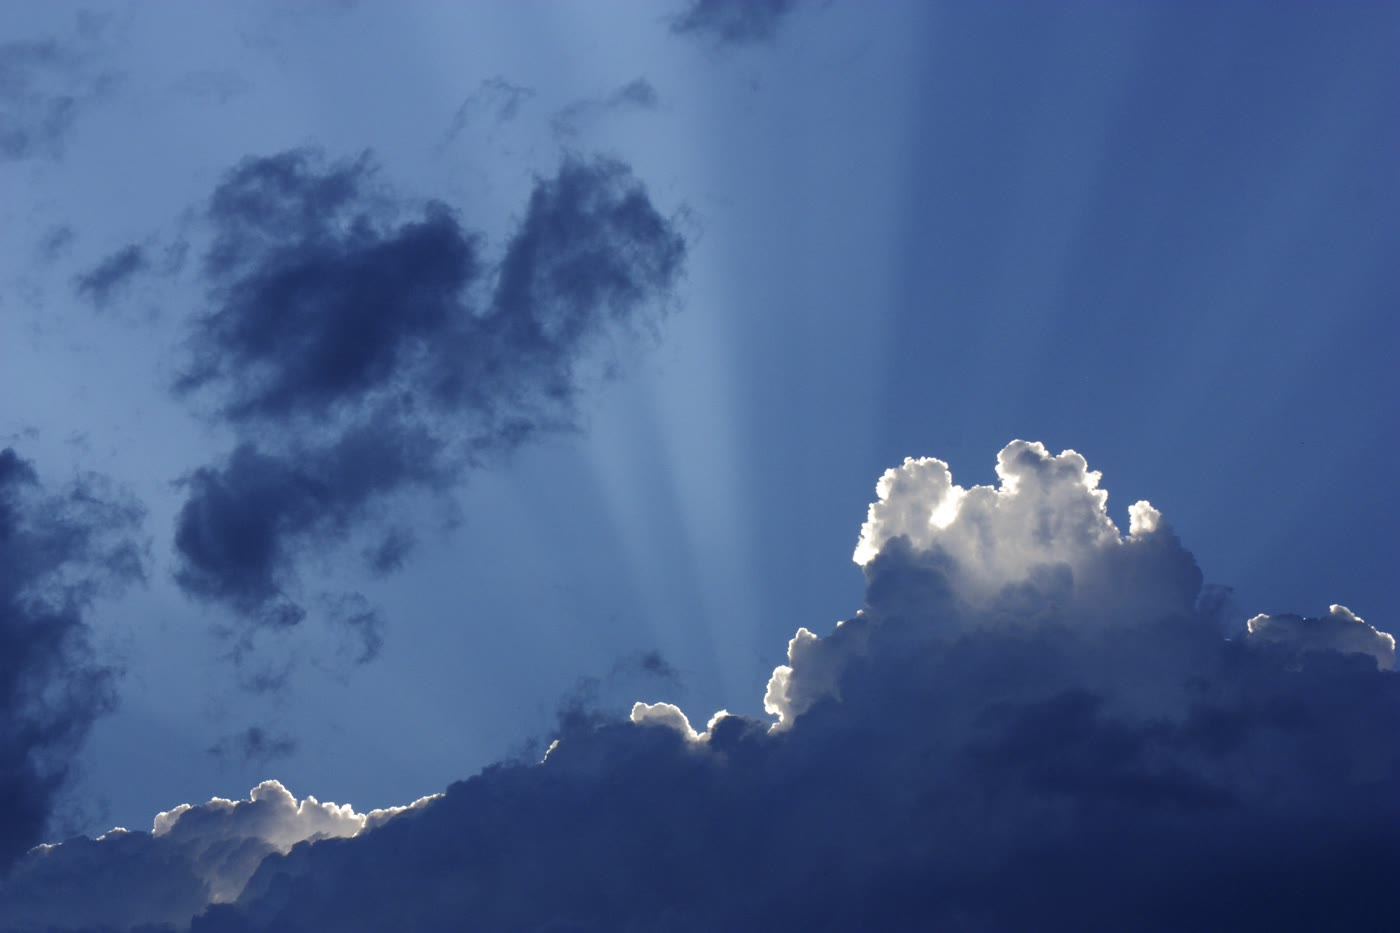
\includegraphics[width=0.55\linewidth]{images/book4/tyndall-sky.jpg}

{\small Rayos de luz a través de un claro entre las nubes: son visibles porque el
\omterm{def:b3:colloids:colloid}{aerosol} del aire, gotitas y polvo, dispersa lateralmente parte de la luz; es el
\omterm{def:b3:colloids:tyndall}{efecto Tyndall} a escala del cielo.}
\end{omfigure}

\section{Estabilidad coloidal}

Dos partículas coloidales siempre se atraen a corta distancia por fuerzas de van der
Waals. En el agua, la mayoría de las partículas llevan además una carga (grupos superficiales
ionizados, iones adsorbidos), rodeada de una \omterm{def:b3:electrode-kinetics:double-layer}{capa difusa} de contraiones, la doble
capa del \cref{ch:b3:electrode-kinetics}. Cuando dos partículas se acercan, sus
\omterm{def:b3:electrode-kinetics:double-layer}{capas difusas} se solapan y se repelen.

\begin{definition}[Potencial zeta]\label{def:b3:colloids:zeta}
El \emph{potencial zeta}\index{potencial zeta} $\zeta$ de una partícula es el potencial
eléctrico en su plano de cizalla, la frontera, dentro de la doble capa, entre
el líquido que se mueve con la partícula y el que no lo hace; se
mide a partir de la velocidad de las partículas en un campo eléctrico
(electroforesis).
\end{definition}

\begin{omfigure}
\begin{tikzpicture}[font=\scriptsize]
  \fill[black!20] (0,0) circle (1.2);
  \foreach \a in {0,30,...,330}{\node at (\a:1.05) {$-$};}
  \draw[omDef, dashed] (0,0) circle (1.55);
  \foreach \a in {15,45,...,345}{\draw[omDef, fill=omDef!15] (\a:1.38) circle (0.11); \node at (\a:1.38) {\tiny$+$};}
  \draw[omThm, thick, densely dotted] (0,0) circle (1.85);
  \foreach \a/\r/\s in {10/2.2/+, 50/2.5/+, 95/2.3/-, 130/2.7/+, 175/2.2/+, 215/2.6/-, 250/2.3/+, 290/2.8/+, 345/2.6/+}{
    \draw[black!60, fill=white] (\a:\r) circle (0.11); \node at (\a:\r) {\tiny$\s$};}
  \draw[->, black!60] (2.6,1.6) node[anchor=west] {capa de Stern} -- (40:1.6);
  \draw[->, omThm] (2.6,-1.4) node[anchor=west] {plano de cizalla: $\zeta$} -- (-30:1.87);
  \node at (0,0) {partícula};
  \node[anchor=west] at (2.9,0.2) {capa difusa};
\end{tikzpicture}

{\small Una partícula cargada negativamente con su doble capa: una capa compacta de Stern
de contraiones, el plano de cizalla justo más allá, donde se define el \omterm{def:b3:colloids:zeta}{potencial
zeta}, y la \omterm{def:b3:electrode-kinetics:double-layer}{capa difusa}, en la que los contraiones superan en número a los
coiones a lo largo de unas pocas \omterm{def:b3:electrode-kinetics:double-layer}{longitudes de Debye}.}
\end{omfigure}

\begin{theorem}[Teoría DLVO]\label{thm:b3:colloids:dlvo}
Para dos esferas de radio $a$ separadas por una distancia $h \ll a$, con potencial de la \omterm{def:b3:electrode-kinetics:double-layer}{capa difusa}
$\psi$ y constante de Hamaker $A$, la energía de interacción es, para potenciales bajos,
\[
  V(h) = 2\pi\varepsilon_r\varepsilon_0a\psi^2\ln\bigl(1 + \eu^{-\kappa h}\bigr) - \frac{Aa}{12h} .
\]
El primer término, la repulsión de doble capa, decae en la \omterm{def:b3:electrode-kinetics:double-layer}{longitud de Debye} $\kappa^{-1}$;
el segundo, la atracción de van der Waals, no depende de la sal. Su suma
presenta una barrera energética a unas pocas \omterm{def:b3:electrode-kinetics:double-layer}{longitudes de Debye} cuando la concentración de sal es
baja, y ninguna por encima de una concentración crítica.
\end{theorem}

\begin{proof}[Demostración parcial]
Ambas formas se admiten (la repulsión, a partir del solapamiento de dos capas de
Gouy--Chapman en la aproximación de Derjaguin; la atracción, sumando las interacciones de London
sobre los dos cuerpos). Aumentar la fuerza iónica aumenta $\kappa$
(\cref{prop:b3:electrode-kinetics:debye-length}): la repulsión se extingue entonces a una
$h$ menor, donde la atracción, que crece como $1/h$, es más fuerte; el máximo
de $V$ disminuye y acaba por desaparecer.
\end{proof}

\begin{omfigure}
\begin{tikzpicture}
\begin{axis}[width=0.72\linewidth, height=5.6cm, xmin=0, xmax=30, ymin=-40, ymax=45,
  axis lines=left, xlabel={distancia $h$ / nm}, ylabel={$V/kT$},
  tick label style={font=\small}, label style={font=\small},
  legend style={font=\scriptsize, draw=none, at={(0.98,0.98)}, anchor=north east}, legend cell align=left]
\addplot[omDef, thick] table[x=h_nm, y=I1] {figdata/out/bachelor-3-dlvo.dat};
\addplot[black!60, thick] table[x=h_nm, y=I10] {figdata/out/bachelor-3-dlvo.dat};
\addplot[omThm, thick] table[x=h_nm, y=I50] {figdata/out/bachelor-3-dlvo.dat};
\addplot[black, thick, dashed] table[x=h_nm, y=I200] {figdata/out/bachelor-3-dlvo.dat};
\draw[black!30] (axis cs:0,0) -- (axis cs:30,0);
\legend{\qty{1}{mM}, \qty{10}{mM}, \qty{50}{mM}, \qty{200}{mM}}
\end{axis}
\end{tikzpicture}

{\small Interacción DLVO de dos partículas de \qty{100}{nm} de radio (modelo: potencial de la \omterm{def:b3:electrode-kinetics:double-layer}{capa
difusa} de \qty{-30}{mV}, constante de Hamaker de \qty{2e-20}{J}) en agua con una sal 1:1. Con \qty{1}{mM},
una barrera de unos $40\,kT$ mantiene separadas las partículas; con \qty{10}{mM}, se reduce a la mitad;
hacia \qty{50}{mM} desaparece y toda colisión es adherente.}
\end{omfigure}

\begin{definition}[Coagulación y estabilización]\label{def:b3:colloids:stability}
La \emph{coagulación}\index{coagulacion@coagulación} es la agregación de partículas coloidales
causada por la pérdida de su repulsión electrostática; la \emph{floculación}\index{floculacion@floculación}
es la agregación en flóculos laxos, a menudo unidos por puentes de polímeros adsorbidos. La
\emph{concentración crítica de coagulación}\index{concentracion critica de coagulacion@concentración crítica de coagulación}
(CCC) de un electrolito es la concentración por encima de la cual un
\omterm{def:b3:colloids:colloid}{coloide} coagula rápidamente. La \emph{estabilización estérica}\index{estabilizacion esterica@estabilización estérica}
mantiene separadas las partículas mediante cadenas de polímero adsorbidas o injertadas,
cuyo solapamiento costaría entropía.
\end{definition}

\begin{proposition}[Regla de Schulze--Hardy]\label{prop:b3:colloids:schulze-hardy}
Para un \omterm{def:b3:colloids:colloid}{coloide} muy cargado, la \omterm{def:b3:colloids:stability}{concentración crítica de coagulación} de un
electrolito varía como la inversa de la sexta potencia de la carga $z$ de sus
contraiones: $\text{CCC} \propto z^{-6}$, en las razones $1 : \frac{1}{64} : \frac{1}{729}$ para $z = 1, 2, 3$.
\end{proposition}

\begin{proof}[Demostración parcial]
Se tratan dos placas planas. A potencial superficial alto, la repulsión de doble capa por
unidad de área tiende a $V_R = (64nkT/\kappa)\eu^{-\kappa h}$, donde $n$ es la densidad numérica del
electrolito $z{:}z$, independiente del potencial (se admite); la atracción es $V_A =
-A/(12\pi h^2)$. En la CCC, la barrera justo se anula: $V = 0$ y $\dd V/\dd h = 0$ a la misma
distancia. Como $\dd V_R/\dd h = -\kappa V_R$ y $\dd V_A/\dd h = -2V_A/h$, las dos condiciones dan
$\kappa V_R = 2V_R/h$, luego $\kappa h = 2$, y entonces $64nkT\eu^{-2}/\kappa = A\kappa^2/(48\pi)$, es decir, $n \propto \kappa^3$. Con
$\kappa^2 = 2nz^2e^2/(\varepsilon kT)$, $\kappa^3 \propto (nz^2)^{3/2}$ y $n \propto n^{3/2}z^3$: por tanto, $n \propto z^{-6}$.
\end{proof}

\begin{omfigure}
\begin{tikzpicture}[font=\small, >=Stealth]
  \foreach \x/\lab/\v in {0/\ce{Na+}/1, 2.6/\ce{Ca^{2+}}/{1/64}, 5.2/\ce{Al^{3+}}/{1/729}}{
    \node at (\x,0) {\lab};
    \node[font=\scriptsize] at (\x,-0.45) {CCC $\times\,\v$};}
  \draw[->, thick, omDef] (-0.8,-0.95) -- (6.0,-0.95) node[midway, below, font=\scriptsize] {dosis menor para coagular un coloide negativo};
\end{tikzpicture}

{\small La regla de Schulze--Hardy para un \omterm{def:b3:colloids:colloid}{coloide} cargado negativamente: la \omterm{def:b3:colloids:stability}{concentración
crítica de coagulación} disminuye con la sexta potencia de la carga del contraión.}
\end{omfigure}

La regla explica por qué las sales de aluminio son tan eficaces para clarificar el agua, y
por qué los ríos depositan su carga de arcilla donde se encuentran con el agua salada del mar.

\begin{method}[Elegir la dosis de un coagulante]\label{met:b3:colloids:coagulant-dose}
\begin{enumerate}
  \item Medir la CCC de un electrolito de referencia para la suspensión (ensayos de jarras
        con dosis crecientes, observando la sedimentación).
  \item Trasladarla al contraión del coagulante con la regla de Schulze--Hardy.
  \item Convertirla en masa de sal por metro cúbico con su fórmula; añadir lo suficiente
        para la hidrólisis y la alcalinidad que consume.
  \item Evitar la sobredosis: unos contraiones muy cargados pueden invertir el signo de
        la carga de las partículas y reestabilizarlas.
\end{enumerate}
\end{method}

\section{Los coloides en acción}

\begin{definition}[Balance hidrófilo--lipófilo]\label{def:b3:colloids:hlb}
El \emph{balance hidrófilo--lipófilo}\index{balance hidrofilo--lipofilo@balance hidrófilo--lipófilo}
(HLB) de un \omterm{def:b3:colloids:surfactant}{tensioactivo no iónico} es, en la escala de Griffin, $20$ veces la fracción
másica de su parte hidrófila: los valores bajos (de 3 a 6) convienen a las \omterm{def:b3:colloids:colloid}{emulsiones} de agua
en aceite, y los altos (de 8 a 18), a las \omterm{def:b3:colloids:colloid}{emulsiones} de aceite en agua y a los detergentes.
\end{definition}

Las \omterm{def:b3:colloids:colloid}{emulsiones} son termodinámicamente inestables, ya que cada gotita lleva
energía interfacial; los emulsionantes las hacen cinéticamente estables al rebajar esa
energía y al añadir una capa repulsiva, cargada o estérica, en torno a cada gotita.
La mayonesa es una \omterm{def:b3:colloids:colloid}{emulsión} de aceite en agua con tanto aceite (unas cuatro quintas partes del
volumen) que las gotitas quedan comprimidas unas contra otras, lo que la convierte en
un sólido blando. Las \omterm{def:b3:colloids:colloid}{espumas} se estabilizan con \omterm{def:b3:colloids:surfactant}{tensioactivos} que frenan el drenaje de las
películas de líquido entre las burbujas; los antiespumantes, a menudo aceites de silicona, se extienden sobre esas
películas y las rompen. En las potabilizadoras, las sales de aluminio o de hierro(III)
coagulan la arcilla y los \omterm{def:b3:colloids:colloid}{coloides} orgánicos que enturbian el agua de los ríos; el
hidróxido que forman arrastra los flóculos al sedimentar. Las nanopartículas metálicas
se mantienen dispersas mediante iones citrato adsorbidos (estabilización electrostática) o mediante cadenas de polímero
unidas por grupos tiol (\omterm{def:b3:colloids:stability}{estabilización estérica}).

\begin{inthelab}[El anillo de du Noüy]
Un anillo de platino, flameado para limpiarlo, cuelga de una balanza y se sumerge
horizontalmente en el líquido; después se levanta lentamente. La fuerza necesaria para sacarlo
a través de la superficie pasa por un máximo; dividida por el doble de la circunferencia del
anillo y corregida según la forma del menisco levantado, da la
\omterm{def:b3:colloids:surface-tension}{tensión superficial}. La medida de una serie de un \omterm{def:b3:colloids:surfactant}{tensioactivo} empieza por la disolución más
diluida, enjuagando el anillo entre muestras.
\end{inthelab}

\begin{safety}{\ghs[0.8cm]{GHS02}\ghs[0.8cm]{GHS05}\ghs[0.8cm]{GHS07}}
% ledger: ghs4:SDS, ghs4:Al2SO43
Dodecilsulfato de sodio en polvo: sólido inflamable, nocivo por ingestión, provoca
lesiones oculares graves e irrita las vías respiratorias; se pesa sin levantar
polvo y con protección ocular. Sulfato de aluminio (\ghs[0.6cm]{GHS05}): provoca lesiones oculares
graves.
\end{safety}

\begin{history}[Tyndall y el ultramicroscopio]
John Tyndall mostró en 1869 que un haz de luz se hace visible en un aire cargado
de partículas finas e invisible en un aire libre de ellas, y que la luz dispersada
es azulada y polarizada. Richard Zsigmondy, que estudiaba el color rojo de los
\omterm{def:b3:colloids:colloid}{soles} de oro, construyó con Henry Siedentopf en 1903 el ultramicroscopio, que ilumina
el \omterm{def:b3:colloids:colloid}{coloide} lateralmente y muestra cada partícula como un punto de luz dispersada
sobre un fondo oscuro, demasiado pequeña para resolverse pero contable. Recibió el
premio Nobel de Química de 1925 por su trabajo sobre los \omterm{def:b3:colloids:colloid}{coloides}.
\end{history}

\section{Ejercicios}

\begin{exercise}[$\star$]\label{exo:b3:colloids:1}
% ledger: st:H2O.25C
Calcúlese la presión en el interior de una burbuja de aire de \qty{1.0}{\micro m} de diámetro en agua a
\qty{25}{\celsius} (exterior: \qty{1.0}{bar}).
\end{exercise}

\begin{exercise}[$\star$]\label{exo:b3:colloids:2}
% ledger: st:H2O.25C
Calcúlese la presión de vapor de una gotita de agua de \qty{10}{nm} de radio respecto del
agua plana a \qty{25}{\celsius} ($V_{\mathrm m} = \qty{18.07}{cm^3/mol}$).
\end{exercise}

\begin{exercise}[$\star$]\label{exo:b3:colloids:3}
Un líquido con $\gamma_{\mathrm{LV}} = \qty{72}{mN/m}$ sobre un sólido con $\gamma_{\mathrm{SV}} = \qty{40}{mN/m}$ y $\gamma_{\mathrm{SL}} =
\qty{20}{mN/m}$ (datos del ejercicio): calcúlese el \omterm{def:b3:colloids:wetting}{ángulo de contacto}. ¿\omterm{def:b3:colloids:wetting}{Moja}?
\end{exercise}

\begin{exercise}[$\star$]\label{exo:b3:colloids:4}
% ledger: eps:H2O.25C
Calcúlese la \omterm{def:b3:electrode-kinetics:double-layer}{longitud de Debye} en agua a \qty{25}{\celsius} para \qty{0.010}{mol/L} de NaCl y de
\ce{MgSO4}.
\end{exercise}

\begin{exercise}[$\star\star$]\label{exo:b3:colloids:5}
Justo por debajo de su CMC, la \omterm{def:b3:colloids:surface-tension}{tensión superficial} de un \omterm{def:b3:colloids:surfactant}{tensioactivo} iónico (1:1, sin sal)
disminuye \qty{12.6}{mN/m} por unidad de $\ln c$ a \qty{25}{\celsius}. Calcúlense el exceso superficial y
el área por molécula.
\end{exercise}

\begin{exercise}[$\star\star$]\label{exo:b3:colloids:6}
\omterm{def:b3:colloids:surface-tension}{Tensiones superficiales} de un \omterm{def:b3:colloids:surfactant}{tensioactivo no iónico}: 52.0, 45.5, 39.1, 33.4, 33.3 y
\qty{33.4}{mN/m} para $\log c = -5.0$, $-4.5$, $-4.0$, $-3.5$, $-3.0$ y $-2.5$ (datos del ejercicio).
Estímese la CMC.
\end{exercise}

\begin{exercise}[$\star\star$]\label{exo:b3:colloids:7}
Para el dodecilsulfato de sodio, tómense $v = \qty{0.350}{nm^3}$, $l = \qty{1.67}{nm}$ y $a_0 = \qty{0.60}{nm^2}$; para un
lípido con dos de esas cadenas, $2v$, la misma $l$ y $a_0 = \qty{0.65}{nm^2}$ (datos del
ejercicio). Predígase la forma de sus agregados.
\end{exercise}

\begin{exercise}[$\star\star$]\label{exo:b3:colloids:8}
Un \omterm{def:b3:colloids:colloid}{sol} cargado negativamente coagula con \qty{60}{mM} de NaCl. Predígase la CCC con \ce{CaCl2}
y con \ce{AlCl3}. ¿Qué haría el \ce{Na3PO4}?
\end{exercise}

\begin{exercise}[$\star\star$]\label{exo:b3:colloids:9}
% ledger: cmc:C12E6
Calcúlese el HLB de Griffin del éter monododecílico del hexaetilenglicol,
\ce{C12H25(OCH2CH2)6OH}, cuya parte hidrófila es $\ce{(OCH2CH2)6OH}$. ¿Es adecuado para una
\omterm{def:b3:colloids:colloid}{emulsión} de aceite en agua?
\end{exercise}

\begin{exercise}[$\star\star\star$]\label{exo:b3:colloids:10}
Una dispersión contiene gotitas de 50 y de \qty{500}{nm} de radio. Usando la \omterm{thm:b3:colloids:kelvin}{ecuación de
Kelvin} aplicada a la solubilidad, explíquese cuáles crecen y cuáles se encogen, y por qué
las \omterm{def:b3:colloids:colloid}{emulsiones} engruesan con el tiempo incluso sin coalescencia.
\end{exercise}

\begin{exercise}[$\star\star\star$]\label{exo:b3:colloids:11}
Demuéstrese a partir de la presión de Laplace que el líquido sube hasta la altura $h = 2\gamma\cos\theta/(\rho gr)$ en un
capilar de radio $r$, y calcúlese para el agua ($\theta = 0$, radio de \qty{0.10}{mm}).
\end{exercise}

\begin{exercise}[$\star\star\star$]\label{exo:b3:colloids:12}
Usando la figura DLVO, explíquese por qué añadir \qty{100}{mM} de NaCl a un \omterm{def:b3:colloids:colloid}{sol} estable con \qty{1}{mM}
lo hace coagular, mientras que añadir un polímero que no se adsorbe no cambia la
barrera, pero un polímero injertado en las partículas puede mantenerlas separadas a cualquier
concentración de sal.
\end{exercise}

% keep the heading with its problem box, which fills a page by itself
\clearpage
\enlargethispage{3\baselineskip}
\section{Problema: clarificar agua turbia con alumbre}

\begin{problem}[{Problema de fin de semana --- clarificar agua turbia con alumbre: la
doble capa de las partículas de arcilla, la barrera DLVO, la regla de Schulze--Hardy y
la dosis de sulfato de aluminio}]
\label{pb:b3:colloids:1}
% ledger: eps:H2O.25C, visc:H2O.25C
Una planta de tratamiento de agua recibe un agua blanda y turbia: partículas de arcilla de
\qty{100}{nm} de radio y densidad \qty{2650}{kg/m^3}, con un potencial de la \omterm{def:b3:electrode-kinetics:double-layer}{capa difusa} de \qty{-30}{mV}, en
agua que contiene \qty{1.0}{mM} de \ce{NaHCO3}. Los ensayos de jarras muestran que las partículas coagulan
rápidamente por encima de \qty{50}{mM} de NaCl (datos del problema). La planta trata \qty{1000}{m^3} por
hora con sulfato de aluminio, $\ce{Al2(SO4)3}$ ($M = \qty{342.3}{g/mol}$).

\medskip\noindent\textbf{Parte I --- Un \omterm{def:b3:colloids:colloid}{coloide} estable.}
\begin{enumerate}
  \item ¿Por qué las partículas de arcilla en el agua llevan una carga negativa?
  \item Calcúlese la fuerza iónica del agua.
  \item Calcúlese su \omterm{def:b3:electrode-kinetics:double-layer}{longitud de Debye}.
  \item Compárese con el radio de las partículas. ¿Qué aproximación de la fórmula DLVO
        justifica esto?
  \item Calcúlese la velocidad de sedimentación de una partícula por la ley de Stokes, $v =
        2\Delta\rho\,gr^2/9\eta$ ($\eta = \qty{0.89}{mPa.s}$), en milímetros por día.
  \item ¿Por qué no se adhieren las partículas unas a otras cuando chocan?
\end{enumerate}

\medskip\noindent\textbf{Parte II --- La barrera DLVO.}
\begin{enumerate}[resume]
  \item Escríbase la energía DLVO de dos partículas.
  \item Léase en la figura la barrera con \qty{1}{mM}, en unidades de $kT$.
  \item ¿Con qué frecuencia cruzarían esa barrera dos partículas que chocan?
  \item ¿Qué le ocurre a la barrera hacia \qty{50}{mM}?
  \item Explíquese por qué añadir sal rebaja la barrera.
\end{enumerate}

\medskip\noindent\textbf{Parte III --- Schulze--Hardy.}
\begin{enumerate}[resume]
  \item Enúnciese la regla.
  \item Predígase la CCC del \ce{Ca^{2+}}.
  \item Predígase la CCC del \ce{Al^{3+}}.
  \item ¿Por qué solo importan los cationes del coagulante para este \omterm{def:b3:colloids:colloid}{coloide}?
  \item ¿Por qué el sulfato del alumbre es casi irrelevante para la \omterm{def:b3:colloids:stability}{coagulación}?
\end{enumerate}

\medskip\noindent\textbf{Parte IV --- La dosis.}
\begin{enumerate}[resume]
  \item Calcúlese la cantidad de \ce{Al^{3+}} necesaria por metro cúbico.
  \item Dedúzcase la cantidad de $\ce{Al2(SO4)3}$ por metro cúbico.
  \item Dedúzcase su masa por metro cúbico.
  \item Dedúzcase la masa usada por hora en la planta.
  \item En el agua, el \ce{Al^{3+}} se hidroliza y reacciona con el hidrogenocarbonato. Escríbase la
        ecuación ajustada que forma \ce{Al(OH)3}.
  \item ¿Qué fracción del hidrogenocarbonato consume la dosis? ¿Cambia mucho el
        pH?
  \item ¿Por qué una sobredosis puede volver a enturbiar el agua?
  \item Enúnciese el resultado: la masa mínima de sulfato de aluminio por metro cúbico.
\end{enumerate}
\end{problem}
